\chapter{Results and Discussions}\thispagestyle{thesisstyle} %chapter head
\graphicspath{{Chapter8/figures/}}
{\setstretch{1.5}
%--------------------------------------------------------------------------------------

All results in this chapter are measured on data that the models did not see during training: later time periods, other corpora, an unseen person's mailbox, and unseen scam-call channels. The numbers were re-measured on the shipped weights on 28 October 2026. Confidence intervals, where given, are 95\% intervals.

\section{Summary of Results}
Table~\ref{tab:headline} gives the headline result of each part of the system.

{\small\setstretch{1.05}
\begin{longtable}{|p{2.5cm}|p{6.0cm}|p{5.7cm}|}
\caption{Headline results}\label{tab:headline}\\
\hline \textbf{Part} & \textbf{Measure} & \textbf{Result} \\ \hline
\endfirsthead
\hline \textbf{Part} & \textbf{Measure} & \textbf{Result} \\ \hline
\endhead
\hline
\endfoot
SMS & Macro-F1 on its own data / on a different corpus; smishing recall on the different corpus & 0.980 / 0.859; 0.786 \\ \hline
Email & Phishing precision / recall, later-in-time split & 0.990 / 0.986 \\ \hline
Email & Phishing precision / recall on 2025--26 mail; false alarms & 0.916 / 0.862; 1.9\% of that legitimate mail, 1.2\% of Enron-Spam legitimate mail \\ \hline
Attachments & Phishing with attachments not cleared as Safe; false alarms added on 1{,}606 real mails & 93.0\% to 93.8\%; none added \\ \hline
Links & ROC-AUC, live phishing links against top sites & 0.920 (recall 0.803 at a 0.5 cut-off) \\ \hline
Fusion & Spam recall on the CEAS day-8 stream & 0.611 to 0.912 \\ \hline
Voice content & Scam calls from seven unseen channels caught; false alarms on 723 real bank calls & 96.2\%; 0.3\% \\ \hline
Synthetic voice & AI voices from 41 unseen tools / Edge-TTS caught, phone channel & 85.8\% / 96.7\% \\ \hline
Synthetic voice & Real voices flagged as AI: video calls / 105 unseen scam calls & 0.6\% / 6.7\% \\ \hline
\end{longtable}
}

\section{SMS}\label{sec:res-sms}
Table~\ref{tab:sms} compares the shipped model with three classical models trained on the same rows, and Figure~\ref{fig:sms} shows the same numbers.

\begin{table}[H]
\caption{SMS: shipped model against baselines trained on the same rows}
\label{tab:sms}
\centering\small\setstretch{1.05}
\begin{tabular}{|p{4.9cm}|c|c|c|c|}
\hline
 & \textbf{In-source} & \multicolumn{3}{c|}{\textbf{Held-out corpus ($n$ = 1{,}780)}} \\ \cline{2-5}
\textbf{Model} & \textbf{macro-F1} & \textbf{macro-F1} & \textbf{Smish. P} & \textbf{Smish. R} \\ \hline
Char 3--5 TF-IDF + LR (shipped) & 0.980 & 0.859 & 0.880 & 0.786 \\ \hline
Char 3--5 TF-IDF + linear SVM & 0.984 & 0.869 & 0.888 & 0.807 \\ \hline
Word 1--2 TF-IDF + LR & 0.971 & 0.815 & 0.871 & 0.647 \\ \hline
Word TF-IDF + naive Bayes & 0.955 & 0.843 & 0.894 & 0.765 \\ \hline
\multicolumn{5}{|l|}{95\% interval of the shipped model: held-out macro-F1 [0.828, 0.886]; smishing recall [0.730, 0.844].} \\ \hline
\end{tabular}
\end{table}

\begin{figure}[H]
\centering
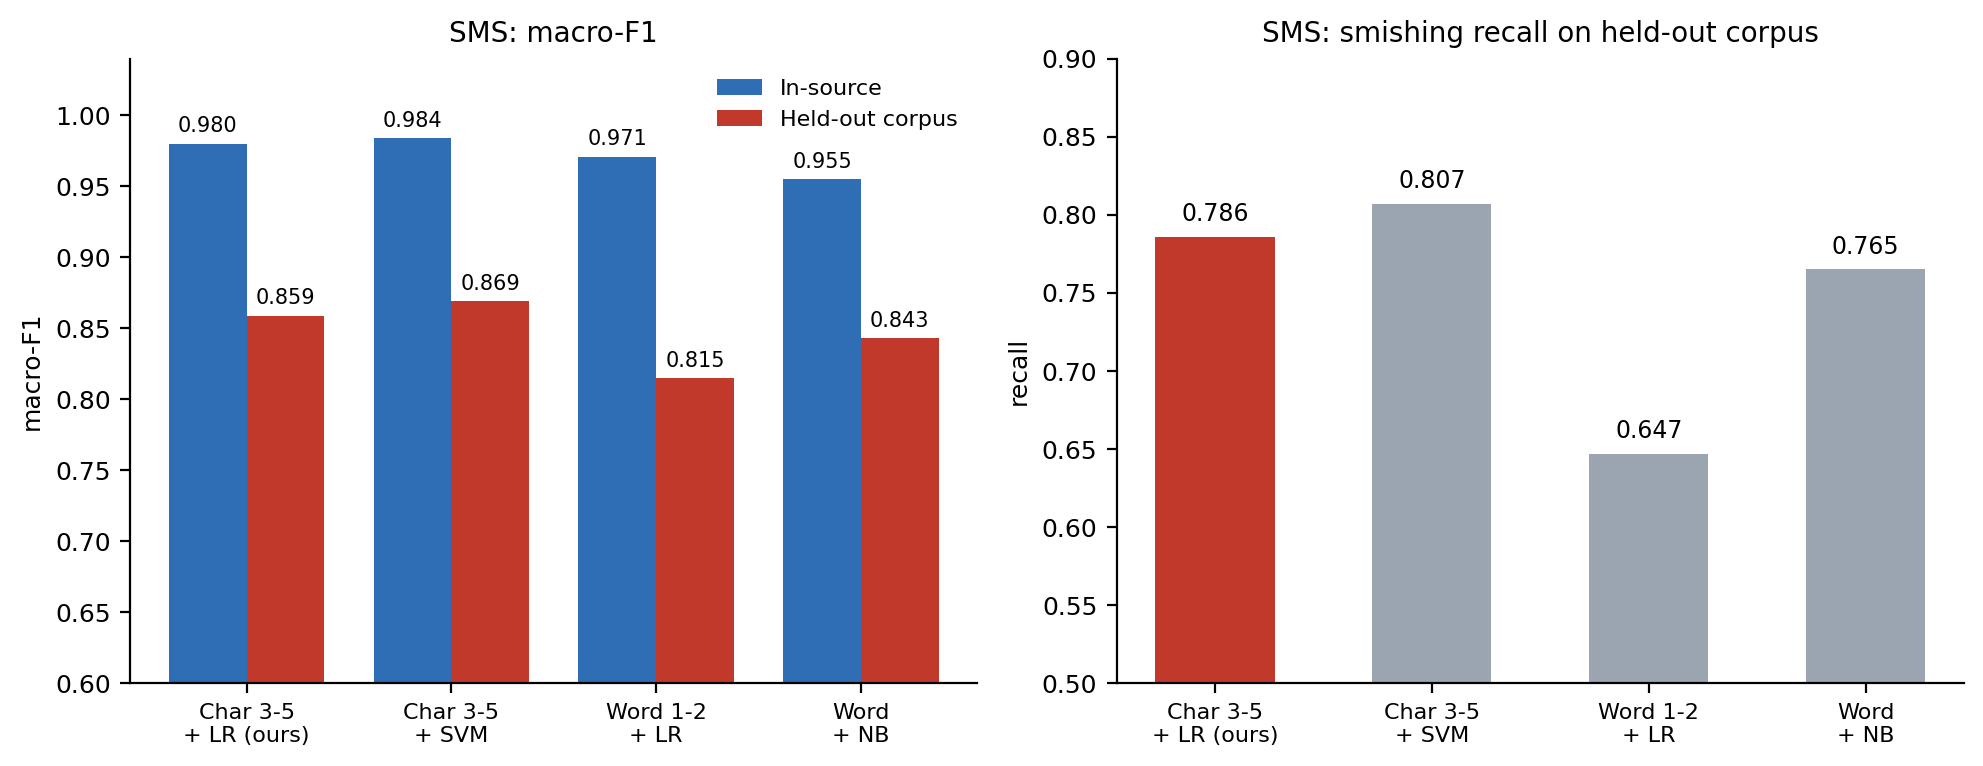
\includegraphics[width=\textwidth]{Chapter8/figures/chart_sms.png}
\caption{SMS results: macro-F1 in-source and on the held-out corpus, and smishing recall on the held-out corpus}
\label{fig:sms}
\end{figure}

\textbf{Discussion.} All four models fall by about the same amount from their own data to the held-out corpus, so the drop is a property of the data and not of one model. The character-based models keep the best smishing recall, and the word-based models lose 4 to 16 points of it. The shipped model fits its vocabulary on public SMS only and uses the private inbox only for weights, because the vocabulary is stored as plain text inside the app. This costs 0.010 of held-out macro-F1 against the otherwise equivalent SVM, and it is the price of making sure that no private word ships in the app. The smishing recall of 0.786 is below the target of 0.90 that was set at the start. Its top features are UK artifacts such as the pound sign and the free-phone prefix ``0800'' from the UCI corpus (Section~\ref{sec:artifacts}), which explains the loss on messages written in another country's conventions. A larger Indian SMS corpus is the real remedy.

\section{Email}\label{sec:res-email}
Table~\ref{tab:email} reports three held-out sets for the shipped DistilBERT model and three classical baselines trained on the same 69{,}927 rows. Figure~\ref{fig:email} shows the results on 2025--26 mail.

\begin{table}[H]
\caption{Email: shipped DistilBERT against baselines on identical rows}
\label{tab:email}
\centering\small\setstretch{1.05}
\begin{tabular}{|p{4.2cm}|c|c|c|c|c|}
\hline
 & \multicolumn{2}{c|}{\textbf{Temporal ($n$ = 9{,}478)}} & \textbf{Cross} & \multicolumn{2}{c|}{\textbf{2025--26 ($n$ = 8{,}725)}} \\ \cline{2-6}
\textbf{Model} & \textbf{F1} & \textbf{Phish P/R} & \textbf{F1} & \textbf{Phish R} & \textbf{Ham FP} \\ \hline
DistilBERT (shipped) & 0.861 & 0.990 / 0.986 & 0.779 & 86.2\% & 1.9\% \\ \hline
Char 3--5 TF-IDF + SVM & 0.860 & 0.995 / 0.984 & 0.754 & 74.9\% & 1.3\% \\ \hline
Word 1--2 TF-IDF + LR & 0.857 & 0.997 / 0.969 & 0.671 & 72.1\% & 0.6\% \\ \hline
Word TF-IDF + naive Bayes & 0.904 & 0.995 / 0.913 & 0.537 & 43.2\% & 0.1\% \\ \hline
\end{tabular}
\end{table}

\begin{figure}[H]
\centering
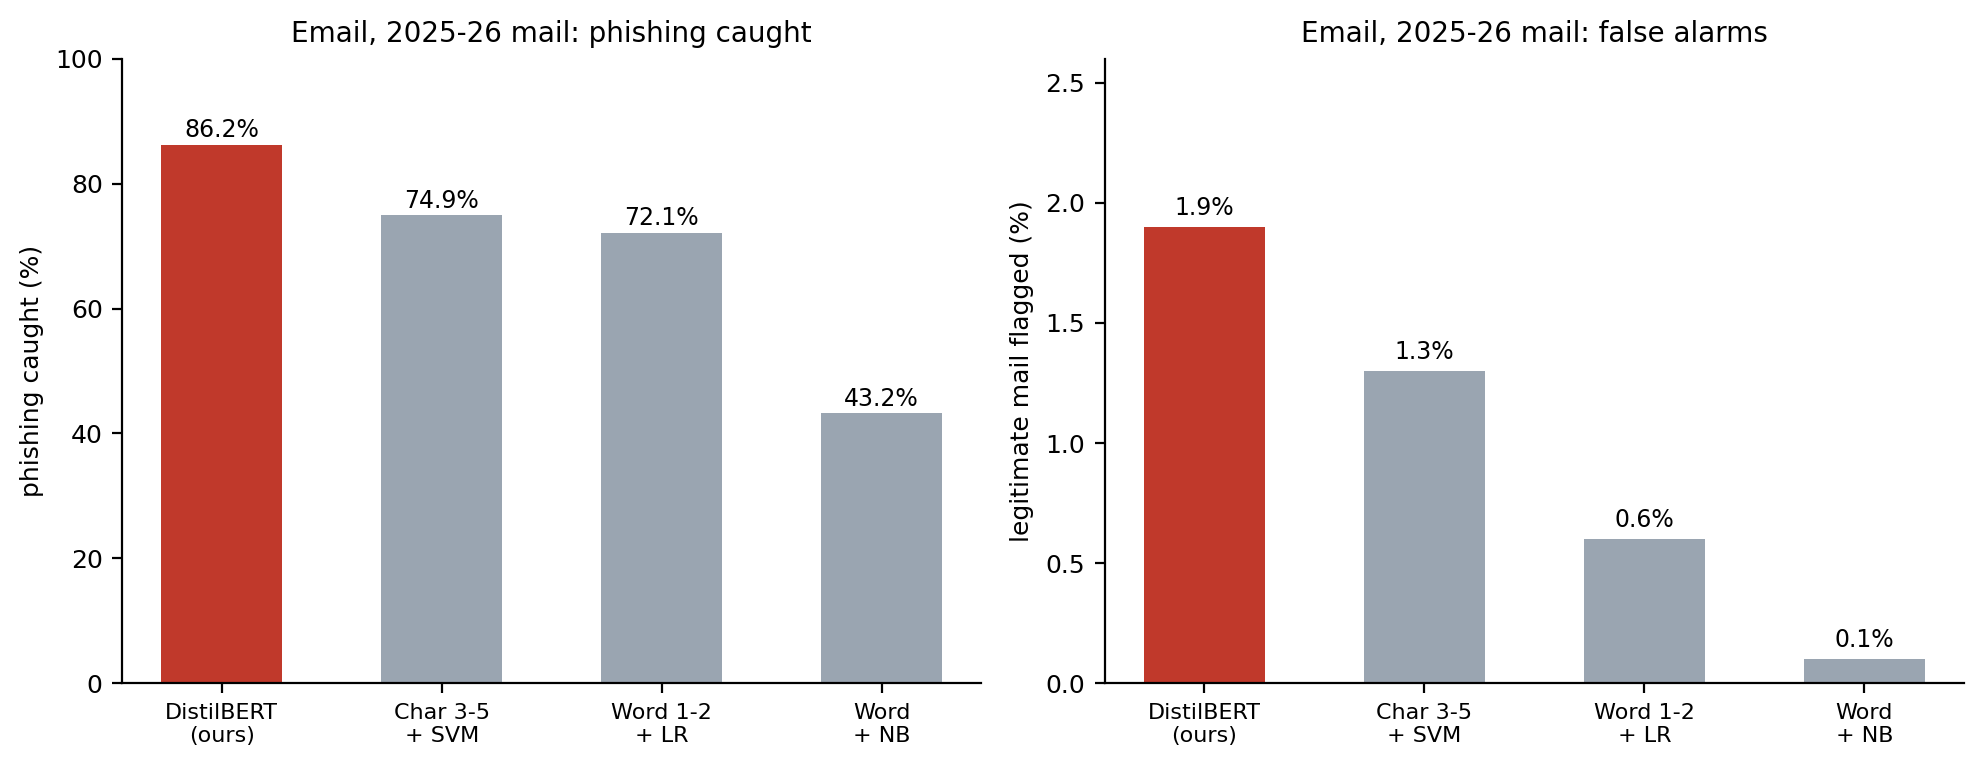
\includegraphics[width=\textwidth]{Chapter8/figures/chart_email.png}
\caption{Email results on 2025--26 mail: phishing caught and legitimate mail flagged}
\label{fig:email}
\end{figure}

\textbf{Discussion.} On the later-in-time split the phishing precision and recall are 0.990 and 0.986 (95\% intervals [0.986, 0.994] and [0.981, 0.991]), but the three-class accuracy is only 0.846: what is missed is spam, not phishing (recall for spam or phishing, 0.747). On 2025--26 mail the model catches 86.2\% of phishing (interval [84.7, 87.8]) and flags 1.9\% of legitimate mail ([1.6, 2.3]\%). It flags 1.2\% of the held-out legitimate mail of Enron-Spam and 4.6\% of the unseen third person's mail. On 2008-era mail the classical baselines are as good or better, and naive Bayes has the best temporal macro-F1 (0.904). The difference appears on data that has moved: on 2025--26 phishing the baselines catch 43 to 75\% against 86.2\% for DistilBERT, and on the unseen corpora their macro-F1 falls to 0.54--0.75. They raise fewer false alarms, mostly because they flag less of everything. The email false alarms of the unseen person are concentrated in one newsletter sender (28 of its 358 mails).

\section{Links}
On 50{,}600 live links (600 phishing, a base rate of 1.19\%) the domain-only XGBoost model reaches a ROC-AUC of 0.920 (interval [0.908, 0.932]). Because ROC-AUC flatters a rare class, the precision--recall view in Figure~\ref{fig:url} matters more: the PR-AUC is 0.585 ([0.544, 0.626]). At the 0.5 cut-off the model catches 80.3\% of phishing but also flags 12.5\% of the benign links (a precision of 0.072), and at a 1\% false-alarm rate it catches 66.2\%. A model that calls everything benign would be 98.8\% accurate, which is why accuracy is not reported. A logistic regression on the same features is close (ROC-AUC 0.928, PR-AUC 0.542), so the features and not the learner carry the result. In the system the link score is one input of three, and Safe Browsing overrides it for known-bad links.

\begin{figure}[H]
\centering
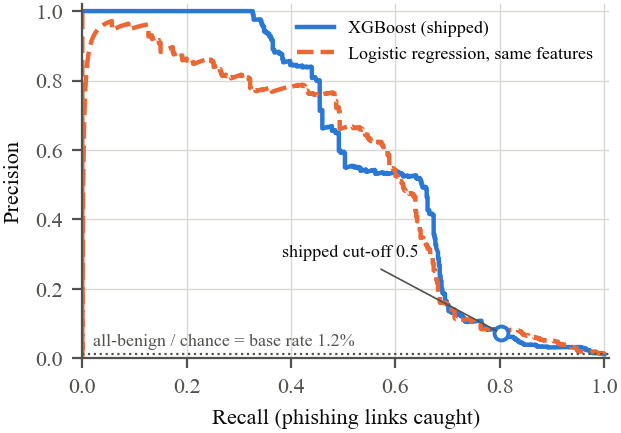
\includegraphics[width=0.85\textwidth]{Chapter8/figures/url_pr.png}
\caption{Precision--recall curve on 50{,}600 live links (OpenPhish against Tranco). Both models see the same 15 host-name features.}
\label{fig:url}
\end{figure}

\section{Attachments}
On 615 phishing mails that carry attachments, the share not cleared as Safe rises from 93.0\% to 93.8\% (interval [91.6, 95.5]) when attachments are checked, and on 1{,}606 real mails with attachments the check adds no false alarms. The gain is small because the content model already catches most of this mail. A check for QR codes was built, but it is switched off: the phishing corpus has no QR codes, so its benefit could not be measured.

\section{Fusion and the Behaviour Engine}\label{sec:res-fusion}
CEAS-08 is the only public corpus that has legitimate mail, spam, real senders and dates, so the behaviour engine is tested on its stream. Profiles are built from 1--7 August and the mail of 8 August is scored once. Figure~\ref{fig:fusion} (left) shows that the spam recall of the content model is 0.611 and that it becomes 0.912 once behaviour may escalate mail that content has cleared.

\begin{figure}[H]
\centering
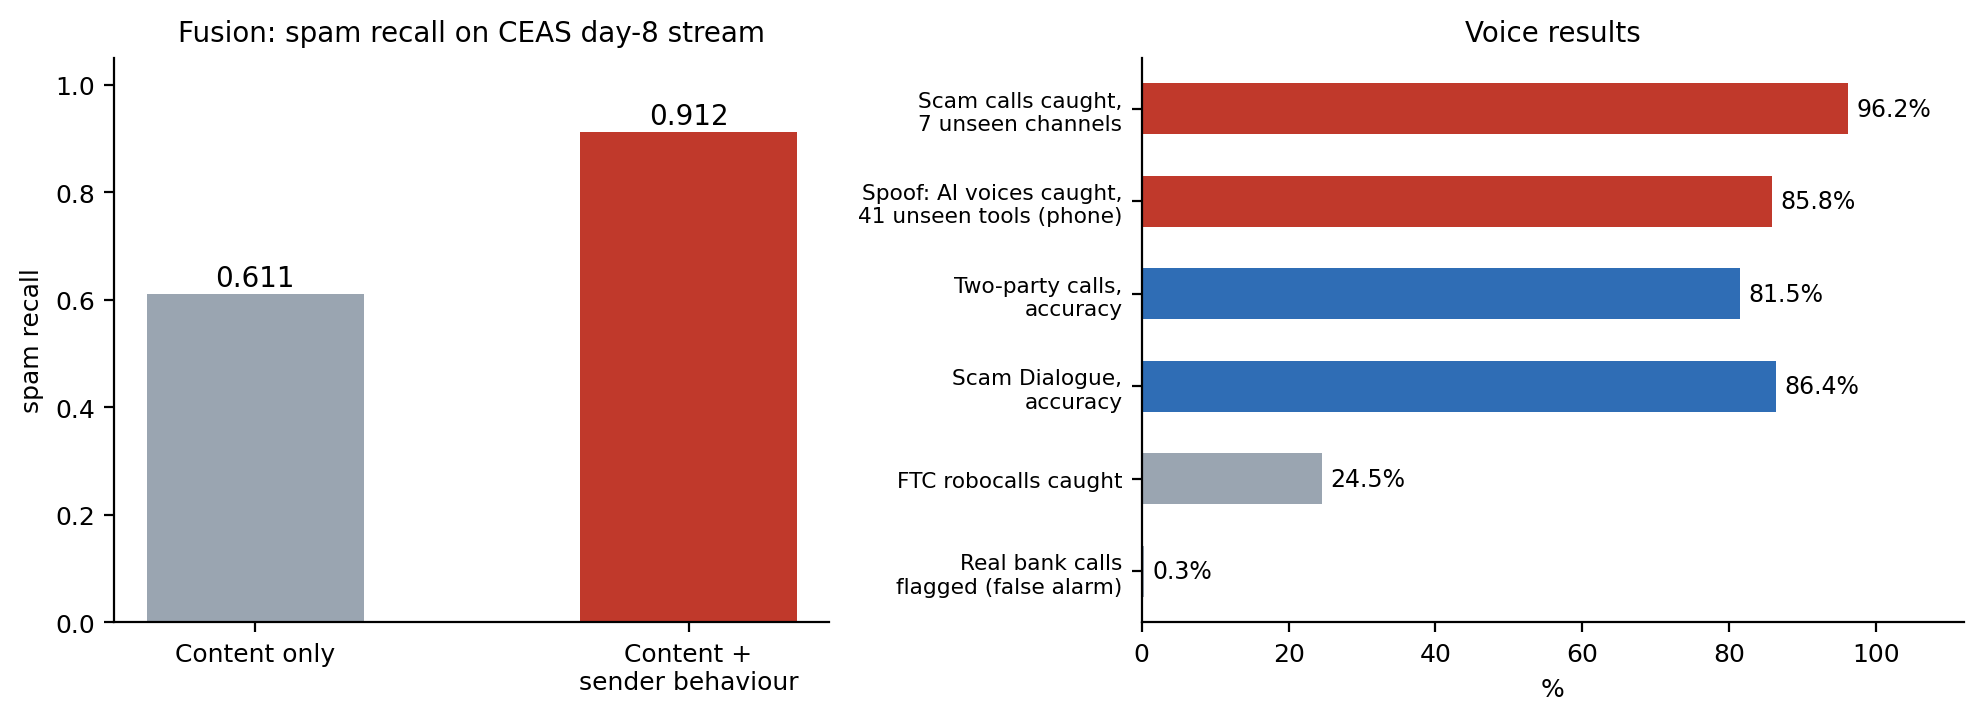
\includegraphics[width=\textwidth]{Chapter8/figures/chart_fusion_voice.png}
\caption{Left: spam recall on the CEAS day-8 stream, with and without sender behaviour. Right: voice results.}
\label{fig:fusion}
\end{figure}

\textbf{Cost.} 8.5\% of the legitimate mail that the content model had cleared is now marked Suspicious (never Phishing). The reasons given for this escalation are almost always ``sender domain never seen before'' and ``no prior history with this sender''.

\textbf{Limits of the claim.} The gain is at this operating point only. As a ranking, the weighted sum is \emph{worse} than the content model alone (AUC 0.963 against 0.990), and a logistic-regression stacker fitted on the first half of the test day does not beat content on the second half (0.947 against 0.974). Behaviour therefore helps by lifting mail that content has cleared, not by reordering mail in general. Almost all the signal is first contact and new domain. Four features (bursts, mass mailing, odd hours and change of writing style) are \emph{inverted} on CEAS (training-window AUC 0.18--0.32) because its recipients are mailing lists, so they carry no weight in the rule. An isolation forest on the same features scores an AUC of 0.595 when fitted on normal traffic and 0.221 when fitted on the whole stream, where half the mail is spam and ``first contact'' is the majority pattern. This is why the behaviour engine uses hand-set rules.

\textbf{Gmail layers.} A failed SPF, DKIM or DMARC check occurs in 35.8\% of the phishing\_pot mail and in 0.5 to 0.8\% of two personal mailboxes. The repeat-sender damping cut the false alarms on the third person's mailbox from 4.6\% to 2.5\% without losing any phishing; it applies to only about a third of legitimate mail, because most real mail links to some other domain. The crowd-report layer is not measured, because no multi-user log exists.

\section{Voice Content}
Table~\ref{tab:voice} reports the content layer on held-out calls.

\begin{table}[H]
\caption{Voice content layer on held-out calls}
\label{tab:voice}
\centering\small\setstretch{1.05}
\begin{tabular}{|p{10.2cm}|p{3.4cm}|}
\hline
\textbf{Test set} & \textbf{Result} \\ \hline
Scam-baiting calls from seven unseen channels ($n$ = 105), caught & 96.2\% \\ \hline
HarperValleyBank half B ($n$ = 723), false alarms & 0.3\% \\ \hline
27 two-party calls, accuracy / AUC & 81.5\% / 0.850 \\ \hline
Scam Dialogue (synthetic, $n$ = 1{,}598), accuracy / AUC & 86.4\% / 0.917 \\ \hline
FTC robocalls ($n$ = 1{,}353), caught (in-source for the act model) & 24.5\% \\ \hline
\end{tabular}
\end{table}

\textbf{Discussion.} The strongest result is on real scam calls from seven channels never used in training (96.2\%, Wilson interval [90.6, 98.5]), against two false alarms in 723 held-out bank calls (0.3\%, [0.1, 1.0]). Two numbers are weak. FTC robocalls are caught only 24.5\% of the time, because a robocall is the bait (``press 1'') and the recording stops before the request. On the 27 two-party calls the score is the maximum over windows, so a 17-minute call gets about 500 chances to cross the band while a short call gets seven. The per-window separation is therefore much weaker than the call-level 81.5\% suggests. Misses are mostly relational scams with no transactional words (a ``relative in trouble'', romance or investment-group openers), and a real police officer saying ``police'' is the one remaining false alarm on the 50 authored test transcripts.

\section{Synthetic Voice}
Figure~\ref{fig:spoof} compares the shipped detector with the earlier one, which was trained on ASVspoof 2019 and 5 only.

\begin{figure}[H]
\centering
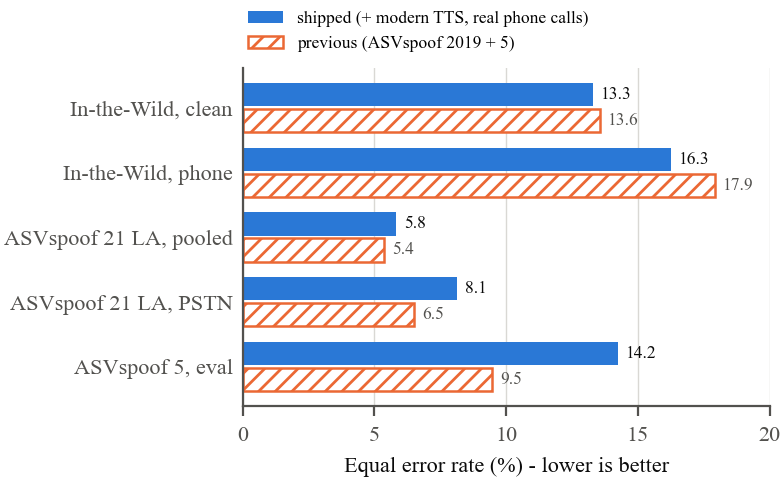
\includegraphics[width=0.9\textwidth]{Chapter8/figures/spoof_eer.png}
\caption{Equal error rate of synthetic-voice detection. The shipped head is trained for unseen modern voices and real phone audio, and is worse on the ASVspoof laboratory sets.}
\label{fig:spoof}
\end{figure}

On modern voices from 41 MLAAD synthesis tools and Edge-TTS that neither head saw, passed through a phone channel, the shipped head catches 85.8\% and 96.7\%, while the earlier head caught 20.0\% of each. It also flags fewer real video-call voices (0.6\% against 2.9\%). The price is visible in the figure: the equal error rate rises on the ASVspoof 2021 phone subset from 6.5\% to 8.1\% (interval [6.3, 10.3]) and on ASVspoof 5 from 9.5\% to 14.2\% ([13.6, 14.9]), and on 105 real scam calls from seven unseen channels the new head flags 6.7\% as synthetic ([3.3, 13.1]) against 1.9\% before. This \emph{failed} one of the rules fixed in advance. The model was promoted by choice, because unseen modern voices are the realistic threat and because the spoof signal can only raise the risk, never decide a verdict alone. On In-the-Wild deepfakes a head trained on ASVspoof 2019 alone reaches an equal error rate of 38.8\%, while the shipped head reaches 13.3\% (clean) and 16.3\% (phone).

\section{Persuasion Head and Explanation Faithfulness}\label{sec:res-faith}
\textbf{Persuasion head.} On true phishing mail the head fires (score of 0.5 or more) for reward in 51.5\%, urgency in 43.4\%, authority in 36.5\%, fear in 10.9\% and scarcity in 10.8\% of the mails. These are firing rates and not accuracy: the labels come from regular expressions and no hand-labelled test set exists. The head is therefore used only to word explanations and never to score.

\textbf{Faithfulness.} A deletion test checks that an explanation names the evidence the model really used. Deleting the three or so words that the SMS explanation names reduces the smishing probability by 0.280 (in-source) and 0.394 (held-out), against 0.030 and 0.040 for three random words, and the verdict flips in 24.8\% and 46.7\% of cases against 2.7\% and 4.8\%. Setting the three top TreeSHAP link features to the benign median reduces the link score by 0.378 and flips 53.7\% of verdicts, against 0.066 and 9.1\% for random features. The explanations are therefore faithful to the models.

\section{Cost}\label{sec:res-cost}
Table~\ref{tab:cost} gives model sizes and the median time to score one message on the development laptop.

\begin{table}[H]
\caption{Model size and median time per message (batch of one)}
\label{tab:cost}
\centering\small\setstretch{1.05}
\begin{tabular}{|p{5.6cm}|p{2.6cm}|p{2.6cm}|p{3.0cm}|}
\hline
\textbf{Component} & \textbf{Size} & \textbf{Disk} & \textbf{Time} \\ \hline
SMS: char 3--5 + LR & 0.19 M weights & 2.6 MB & 0.9 ms (CPU) \\ \hline
Links: XGBoost, 400 trees & 15 features & 2.0 MB & 3.6 ms (CPU) \\ \hline
Phone assets (SMS + links) & -- & 2.1 MB & on the phone \\ \hline
Email: DistilBERT + persuasion head & 66 M & 266 MB & 15.0 ms (GPU) \\ \hline
Voice act model (DistilBERT) & 67 M & 269 MB & 13.1 ms (GPU) \\ \hline
Synthetic voice: XLS-R 300M + LR head & 315 M & 1.2 GB (shared encoder; the trained head is 0.1 MB) & 36.2 ms per 4 s clip \\ \hline
Whisper small (half precision) & 244 M & -- & 3.1 s per audio minute \\ \hline
\end{tabular}
\end{table}

The SMS and link models together take 2.1 MB on the phone and score a message in a few milliseconds on a CPU. Whisper transcribes at 0.051 times real time (3.1 s per minute of audio), so the voice path keeps up with a live call on one consumer GPU.

\section{Comparison with Existing Systems}
There are two fair ways to compare. The first is against standard models trained on the \emph{same rows}, which is what Tables~\ref{tab:sms} and~\ref{tab:email} do. The classical models are as good as the deep model on old data and fall behind on new data: on 2025--26 phishing they catch 43 to 75\% against 86.2\%. The second is by what each system can do, as in Table~\ref{tab:compare}, using the survey of Chapter~2.

\begin{table}[H]
\caption{Capabilities compared with the prior work surveyed}
\label{tab:compare}
\centering\small\setstretch{1.05}
\begin{tabular}{|p{3.7cm}|p{5.0cm}|p{5.3cm}|}
\hline
\textbf{Capability} & \textbf{Typical prior work} & \textbf{This project} \\ \hline
Channels & One of email, SMS or voice & All three, one verdict \\ \hline
Sender behaviour & Not used & Profile per sender and caller \\ \hline
Evaluation & Mostly random splits of one data set & Time, person, corpus and channel splits; rules set in advance \\ \hline
Explanation & Some use LIME or SHAP on email & Reasons on every verdict, tested for faithfulness \\ \hline
Phone deployment & Server side & SMS on the phone, no internet permission \\ \hline
Synthetic voice & A separate line of work & A signal inside the call verdict \\ \hline
Weak results & Seldom reported & Reported, with intervals \\ \hline
\end{tabular}
\end{table}

\section{Corpus Artifacts}\label{sec:artifacts}
The most repeated finding of the project is that a high score often measured the \emph{data set}. Table~\ref{tab:artifacts} lists every case found. Each gave a convincing number, and each was caught only by an ablation, an outside test set, or by checking what a single feature scores alone. This is the pitfall that Arp et al.~\cite{arp2022dos} call spurious correlation; the table adds measured instances for each channel.

{\small\setstretch{1.05}
\begin{longtable}{|p{0.6cm}|p{3.0cm}|p{5.3cm}|p{4.8cm}|}
\caption{Corpus artifacts found: what the feature really encoded, and what it cost}\label{tab:artifacts}\\
\hline \textbf{\#} & \textbf{Where} & \textbf{What the model learned} & \textbf{Measured effect} \\ \hline
\endfirsthead
\hline \textbf{\#} & \textbf{Where} & \textbf{What the model learned} & \textbf{Measured effect} \\ \hline
\endhead
\hline
\endfoot
1 & PhiUSIIL links & 100\% of legitimate URLs are HTTPS with no path & Scheme and path features: AUC 0.331 on live links (below chance) \\ \hline
2 & CEAS-08 has-a-link flag & 2008 legitimate mail was link-heavy list digests; spam was plain text & The flag alone: AUC 0.395; a stacker shows a false 0.986 \\ \hline
3 & CEAS-08 labels & Its ``phishing'' label means spam & The model catches 30.9\% of real (Nazario) phishing \\ \hline
4 & Email phishing source & Public phishing corpora share one style & Public-only model: 98.9\% on its own source, 42.6\% on 2025--26 mail \\ \hline
5 & Enron against modern legitimate mail & Era and mail software, not intent & Surface features separate Enron from 2025 mail at AUC 0.885 \\ \hline
6 & Speech transcripts & Scam = machine transcript; legitimate = typed text & AUC 1.000 in-source; 0.576 on real calls \\ \hline
7 & UCI SMS & UK currency and free-phone numbers mark scams & Top features ``pound sign 1'' and ``0800''; recall drops on other corpora \\ \hline
8 & Indian SMS spam class & No Indian marketing messages existed & Offer plus link read as smishing; a real coupon scored 0.631 \\ \hline
9 & Indian SMS metadata & A ``platform found'' column (Call or Telegram = 100\% fraud) & A free label; the column is withheld \\ \hline
10 & Indian SMS templates & 3{,}200 rows from about 1{,}400 templates & Random split gives TF-IDF F1 0.99; a grouped split is used \\ \hline
11 & Mishra--Soni releases & The 10{,}191-row file is a rebalanced copy of the 5{,}971-row one & Train and test leak unless de-duplicated \\ \hline
12 & CEAS behaviour & Recipients are mailing lists & Burst, mass-mail and hour features are inverted (AUC 0.18--0.32) \\ \hline
13 & Spoof, clean training & Clean real speech against clean fakes & Real voices through a phone line score 0.841 ``fake'' \\ \hline
\end{longtable}
}

\section{Error Analysis and Threats to Validity}
\textbf{Errors.} SMS errors on the held-out corpus are mostly smishing written in another country's conventions (currency, short codes) that the UK-heavy training mix has not seen. Email false alarms on the unseen person are concentrated in one newsletter sender, and spam is missed when it reads like a newsletter, which is a consent problem and not a content one. Voice misses are relational scams with no transactional words. In the functional tests of Chapter~7, three short authored emails from an unknown sender (a loan offer, a sign-in notice and a subscription notice) were called Phishing, which shows the same weakness in short legitimate notices.

\textbf{Threats to validity.}
\begin{enumerate}
\item Two of the three mailboxes and the SMS inbox belong to team members, and the third mailbox shaped the final email recipe, so it is not fully independent.
\item The held-out SMS corpus shares an origin with a training release and is de-duplicated by exact text only.
\item The victims in the scam-baiting calls are performers. The act model scores only the caller's turns, but the choice of channels is ours.
\item The behaviour rules for SMS and calls are not measured, because no public corpus has sender or caller fields.
\item Crowd reports are not measured.
\item A second attempt was made against the scam-baiting set, which weakens that test as evidence.
\end{enumerate}

\section{Discussion}
Four conclusions follow from the measurements.
\begin{enumerate}
\item \textbf{Behaviour helps where content cannot.} Spam recall rose from 0.611 to 0.912. The cost is a larger share of legitimate mail marked Suspicious, which is acceptable for a warning band and not for a block.
\item \textbf{Content models hold up on later and unseen data for email and calls} (0.986 phishing recall on the later split, 96.2\% of unseen scam calls), \textbf{and degrade honestly where the data shifted most} (SMS, 0.786).
\item \textbf{Good scores need an evaluation that can fail.} The thirteen artifacts of Table~\ref{tab:artifacts} would each have been a headline number under a random split.
\item \textbf{The weak points are known.} They are SMS recall on other countries' messages, short genuine notices in the email model, the low precision of the link model on a rare class, and the unmeasured behaviour rules for SMS and calls.
\end{enumerate}

\section{Summary}
The system meets most of its objectives on data it has not seen. Its strongest results are for email on later data, scam calls on unseen channels and the gain from sender behaviour. Its weakest are smishing recall on another corpus, short genuine email notices and the link model's precision, and these are reported openly.

%--------------------------------------------------------------------------------------
}
